\documentclass[../main.tex]{subfiles}
\begin{document}

\chapter{Системийн шинжилгээ, зохиомж}

Энэхүү бүлэгт бараа таних болон аудитын автомат системийн бизнесийн шинжилгээ, системийн шаардлагууд, ажлын явц (use case), технологийн судалгаа болон техникийн архитектурын зохиомжийг тодорхойлно.

%==============================================================================
% 2.1 БИЗНЕСИЙН ОРОЛЦОГЧИД
%==============================================================================
\section{Бизнесийн оролцогчид}

Жижиглэн худалдааны бараа материалын тооллого, аудитын үйл ажиллагаанд дараах оролцогчид оролцоно:

\begin{table}[H]
\centering
\caption{Бизнесийн оролцогчдын тодорхойлолт}
\label{tab:stakeholders}
\begin{tabular}{|p{3.5cm}|p{10cm}|}
\hline
\textbf{Оролцогч} & \textbf{Үүрэг, хариуцлага} \\
\hline
Дэлгүүрийн менежер & Өдөр тутмын бараа материалын нөөцийг хянах, захиалга өгөх, лангууны зохион байгуулалтыг шийдвэрлэх \\
\hline
Лангууны ажилтан & Бараа өрөх, лангууг цэгцлэх, дутагдсан барааг нөхөн дүүргэх \\
\hline
Түгээгч (Merchandiser) & Бараа нийлүүлэх, лангууны байрлалыг шалгах, planogram-тай тулгах \\
\hline
Бөөний нийлүүлэгч & Бараа нийлүүлэх, нөөцийн түвшинг хянах, дахин захиалгын шаардлагыг тодорхойлох \\
\hline
Аудитор & Бараа материалын тооллого хийх, зөрүү илрүүлэх, тайлан бэлтгэх \\
\hline
Системийн админ & Системийн тохиргоо хийх, хэрэглэгчийн эрх удирдах, ML загварыг шинэчлэх \\
\hline
\end{tabular}
\end{table}

%==============================================================================
% 2.2 БИЗНЕСИЙН ҮЙЛ АЖИЛЛАГААНЫ ШИНЖИЛГЭЭ
%==============================================================================
\section{Бизнесийн үйл ажиллагааны шинжилгээ}

\subsection{Одоогийн байдал (As-Is)}

Монголын жижиглэн худалдааны салбарт бараа материалын тооллого, аудит хийх уламжлалт арга нь дараах үе шатуудаас бүрдэнэ:

\begin{enumerate}
    \item \textbf{Гар аргаар тоолох:} Ажилтан лангуу бүрт очиж бараа бүрийг нэг нэгээр нь тоолж, цаасан маягт эсвэл Excel хүснэгтэд бичиж тэмдэглэнэ.
    \item \textbf{Мэдээлэл нэгтгэх:} Олон ажилтны бичсэн тэмдэглэлийг нэгтгэж, нийт тооллогын тайлан гаргана.
    \item \textbf{Системд оруулах:} Тоологдсон мэдээллийг ERP эсвэл POS системд гараар оруулна.
    \item \textbf{Зөрүү шалгах:} Системийн бүртгэлтэй харьцуулж, зөрүүг илрүүлнэ.
\end{enumerate}

\begin{figure}[H]
\centering
\begin{tikzpicture}[
    node distance=1.2cm,
    process/.style={rectangle, draw, fill=gray!20, minimum width=2.8cm, minimum height=0.8cm, align=center, rounded corners, font=\footnotesize},
    arrow/.style={->, thick, >=stealth}
]
% Current process
\node[process] (s1) at (0, 0) {Гар аргаар\\тоолох};
\node[process] (s2) at (3.5, 0) {Цаасанд\\бичих};
\node[process] (s3) at (7, 0) {Мэдээлэл\\нэгтгэх};
\node[process] (s4) at (10.5, 0) {Системд\\оруулах};
\node[process] (s5) at (7, -1.5) {Зөрүү\\шалгах};
\node[process] (s6) at (3.5, -1.5) {Тайлан\\гаргах};

\draw[arrow] (s1) -- (s2);
\draw[arrow] (s2) -- (s3);
\draw[arrow] (s3) -- (s4);
\draw[arrow] (s4) -- (s5);
\draw[arrow] (s5) -- (s6);

\node[font=\small, above] at (5.25, 0.8) {\textbf{Уламжлалт тооллогын үйл явц (4-8 цаг)}};
\end{tikzpicture}
\caption{Одоогийн бараа материалын тооллогын үйл явц}
\label{fig:current_process}
\end{figure}

\subsection{Асуудлууд}

Уламжлалт аргын дараах асуудлуудыг судалгаагаар тодорхойлов:

\begin{table}[H]
\centering
\caption{Уламжлалт аргын асуудлууд}
\label{tab:problems}
\begin{tabular}{|p{3cm}|p{5cm}|p{5.5cm}|}
\hline
\textbf{Асуудлын төрөл} & \textbf{Тодорхойлолт} & \textbf{Үр дагавар} \\
\hline
Цаг хугацаа & Нэг дэлгүүрийн тооллого 4-8 цаг үргэлжилнэ & Бүтээмж буурах, хөдөлмөрийн зардал өндөр \\
\hline
Хүний алдаа & Гараар тоолоход 2-5\% алдаа гарна \cite{zebra_study} & Нөөцийн тооцоо буруу, алдагдал \\
\hline
Мэдээлэл тархмал & Цаасан маягт, Excel файлууд нэгдсэн системгүй & Мэдээлэл алдагдах, хайх хүндрэлтэй \\
\hline
Бодит цаг & Тооллого дууссаны дараа л мэдээлэл шинэчлэгддэг & Бодит байдалтай таарахгүй \\
\hline
Зардал өндөр & Тусгай ажилтан, нэмэлт цагийн хөлс шаарддаг & Ашигт ажиллагаа буурна \\
\hline
\end{tabular}
\end{table}

McKinsey судалгаагаар жижиглэн худалдааны компаниуд нөөцийн зөрүүгээс болж жилд дунджаар 4.1\%-ийн борлуулалтын алдагдалтай тулгардаг \cite{mckendrick_ai}. IHL Group-ийн тайланд дэлхий даяар $1.1 их наяд долларын алдагдал бараа материалын буруу удирдлагаас үүдэлтэй гэж тооцоолсон \cite{ihl_report}.

\subsection{Санал болгож буй шийдэл (To-Be)}

Энэхүү төсөл нь компьютерын хараа (Computer Vision) болон гүн сургалтын (Deep Learning) технологи ашиглан дээрх асуудлуудыг шийдвэрлэнэ:

\begin{figure}[H]
\centering
\begin{tikzpicture}[
    node distance=1.2cm,
    process/.style={rectangle, draw, fill=blue!20, minimum width=2.8cm, minimum height=0.8cm, align=center, rounded corners, font=\footnotesize},
    arrow/.style={->, thick, >=stealth}
]
% New process
\node[process, fill=cyan!30] (s1) at (0, 0) {Зураг авах\\(3 секунд)};
\node[process, fill=green!30] (s2) at (3.5, 0) {AI илрүүлэлт\\(1 секунд)};
\node[process, fill=yellow!30] (s3) at (7, 0) {Автомат\\аудит};
\node[process, fill=orange!30] (s4) at (10.5, 0) {Үр дүн\\харуулах};

\draw[arrow] (s1) -- (s2);
\draw[arrow] (s2) -- (s3);
\draw[arrow] (s3) -- (s4);

\node[font=\small, above] at (5.25, 0.8) {\textbf{Автомат тооллогын үйл явц (5 секунд)}};
\end{tikzpicture}
\caption{Санал болгож буй автомат тооллогын үйл явц}
\label{fig:proposed_process}
\end{figure}

\textbf{Шийдлийн үндсэн санаа:}
\begin{enumerate}
    \item Гар утас эсвэл камераар лангууны зураг авна
    \item YOLOv8 загвар зураг дээрх бүх барааг таньж тоолно
    \item Системд бүртгэлтэй ``байх ёстой'' тоотой автоматаар харьцуулна
    \item Зөрүү илэрвэл PASS/WARNING/FAIL статус гаргана
\end{enumerate}

\subsection{Хүлээгдэж буй үр дүн}

\begin{table}[H]
\centering
\caption{Хүлээгдэж буй үр дүнгийн харьцуулалт}
\label{tab:expected_results}
\begin{tabular}{|p{4cm}|p{4cm}|p{4.5cm}|}
\hline
\textbf{Хэмжүүр} & \textbf{Уламжлалт арга} & \textbf{AI систем} \\
\hline
Нэг лангууны тооллого & 15-30 минут & 5-10 секунд \\
\hline
Тооллогын алдаа & 2-5\% & <1\% (загварын нарийвчлалаас хамаарна) \\
\hline
Шаардлагатай ажилтны тоо & 2-4 хүн & 1 хүн \\
\hline
Өдөрт хийх боломжтой тооллого & 2-3 удаа & Хязгааргүй \\
\hline
Мэдээлэл боловсруулах хугацаа & 1-2 өдөр & Шууд (real-time) \\
\hline
\end{tabular}
\end{table}

%==============================================================================
% 2.3 СИСТЕМИЙН ШААРДЛАГУУД
%==============================================================================
\section{Системийн шаардлагууд}

\subsection{Функциональ шаардлагууд}

Функциональ шаардлага (ФШ) нь систем ямар үйлдлүүдийг гүйцэтгэх ёстойг тодорхойлно.

\begin{longtable}{|p{1.2cm}|p{4cm}|p{8cm}|}
\caption{Функциональ шаардлагууд} \label{tab:functional_requirements} \\
\hline
\textbf{Код} & \textbf{Шаардлага} & \textbf{Тодорхойлолт} \\
\hline
\endfirsthead
\hline
\textbf{Код} & \textbf{Шаардлага} & \textbf{Тодорхойлолт} \\
\hline
\endhead
\hline
\endfoot
\multicolumn{3}{|c|}{\textbf{Зураг оруулах модуль}} \\
\hline
ФШ100 & Зураг авах & Хэрэглэгч гар утасны камераар зураг авч системд илгээх боломжтой байна \\
\hline
ФШ110 & Зураг сонгох & Хэрэглэгч төхөөрөмжийн санах ойгоос зураг сонгон илгээх боломжтой байна \\
\hline
ФШ120 & Зураг урьдчилан харах & Илгээхээс өмнө зургийг урьдчилан харах боломжтой байна \\
\hline
\multicolumn{3}{|c|}{\textbf{Бараа илрүүлэх модуль}} \\
\hline
ФШ200 & Бараа таних & Систем зураг дээрх бүх барааг YOLOv8 загвараар таньж тодорхойлно \\
\hline
ФШ210 & Итгэлцлийн оноо & Илрүүлсэн бараа бүрийн итгэлцлийн оноог (confidence score) харуулна \\
\hline
ФШ220 & Bounding box & Илрүүлсэн барааны байрлалыг bounding box-оор харуулна \\
\hline
ФШ230 & Тоо гаргах & Ангилал тус бүрээр нийт хэдэн бараа илрүүлснийг тоолж гаргана \\
\hline
\multicolumn{3}{|c|}{\textbf{Аудит модуль}} \\
\hline
ФШ300 & Аудит хийх & Илрүүлсэн тоог ``байх ёстой'' тоотой харьцуулж аудит хийнэ \\
\hline
ФШ310 & Статус тодорхойлох & Тохирлын хувиас хамаарч PASS/WARNING/FAIL статус гаргана \\
\hline
ФШ320 & Зөрүү харуулах & Аль бараа хэдээр зөрсөн, дутуу эсвэл илүү болохыг харуулна \\
\hline
ФШ330 & Аудит хадгалах & Аудитын үр дүнг MongoDB-д хадгална \\
\hline
\multicolumn{3}{|c|}{\textbf{Бараа бүртгэлийн модуль}} \\
\hline
ФШ400 & Бараа нэмэх & Шинэ барааны мэдээлэл (нэр, ангилал, ``байх ёстой'' тоо) бүртгэнэ \\
\hline
ФШ410 & Бараа засах & Бүртгэлтэй барааны мэдээллийг засварлана \\
\hline
ФШ420 & Бараа устгах & Барааны бүртгэлийг устгана \\
\hline
ФШ430 & Бараа хайх & Нэр, ангиллаар бараа хайх боломжтой байна \\
\hline
\multicolumn{3}{|c|}{\textbf{Түүх, тайлан модуль}} \\
\hline
ФШ500 & Илрүүлэлтийн түүх & Өмнөх илрүүлэлтүүдийг харах боломжтой байна \\
\hline
ФШ510 & Аудитын түүх & Өмнөх аудитуудыг харах боломжтой байна \\
\hline
ФШ520 & Статистик & Нийт аудитын тоо, амжилтын хувь зэрэг статистик харуулна \\
\hline
\end{longtable}

\subsection{Функциональ бус шаардлагууд}

Функциональ бус шаардлага (ФБШ) нь системийн чанар, гүйцэтгэлийн шалгууруудыг тодорхойлно.

\begin{longtable}{|p{1.2cm}|p{3.5cm}|p{8.5cm}|}
\caption{Функциональ бус шаардлагууд} \label{tab:non_functional_requirements} \\
\hline
\textbf{Код} & \textbf{Шаардлага} & \textbf{Тодорхойлолт} \\
\hline
\endfirsthead
\hline
\textbf{Код} & \textbf{Шаардлага} & \textbf{Тодорхойлолт} \\
\hline
\endhead
\hline
\endfoot
\multicolumn{3}{|c|}{\textbf{Гүйцэтгэл (Performance)}} \\
\hline
ФБШ100 & Хариу өгөх хугацаа & Нэг зургийн илрүүлэлт 2 секундээс бага хугацаанд дуусна \\
\hline
ФБШ110 & Зэрэгцээ хүсэлт & Систем нэгэн зэрэг 50 хүсэлт хүлээн авч боловсруулна \\
\hline
ФБШ120 & Загварын хэмжээ & ML загвар 50MB-аас бага байна (гар утсанд ачаалах боломжтой) \\
\hline
\multicolumn{3}{|c|}{\textbf{Нарийвчлал (Accuracy)}} \\
\hline
ФБШ200 & mAP@50 & Загварын mAP@50 нарийвчлал 80\%-аас дээш байна \\
\hline
ФБШ210 & Precision & Precision 85\%-аас дээш байна \\
\hline
ФБШ220 & Recall & Recall 80\%-аас дээш байна \\
\hline
\multicolumn{3}{|c|}{\textbf{Хэрэглэхэд хялбар (Usability)}} \\
\hline
ФБШ300 & Интерфейс & 3 товшилтоос бага үйлдлээр зураг илгээх боломжтой байна \\
\hline
ФБШ310 & Суралцах хугацаа & Шинэ хэрэглэгч 5 минутын дотор системийг ашиглаж сурна \\
\hline
ФБШ320 & Хэл & Монгол хэлээр интерфейстэй байна \\
\hline
\multicolumn{3}{|c|}{\textbf{Найдвартай байдал (Reliability)}} \\
\hline
ФБШ400 & Uptime & Системийн uptime 99\%-аас дээш байна \\
\hline
ФБШ410 & Алдааны удирдлага & Алдаа гарсан үед хэрэглэгчид ойлгомжтой мэдэгдэл харуулна \\
\hline
ФБШ420 & Өгөгдөл хадгалах & MongoDB replica set ашиглан өгөгдлийн нөөц хийнэ \\
\hline
\multicolumn{3}{|c|}{\textbf{Өргөтгөх боломж (Scalability)}} \\
\hline
ФБШ500 & Хэвтээ өргөтгөл & Docker container ашиглан хэвтээ өргөтгөл хийх боломжтой байна \\
\hline
ФБШ510 & Шинэ бараа нэмэх & Шинэ ангиллын бараа нэмэхэд загварыг дахин сургах боломжтой байна \\
\hline
\end{longtable}

\subsection{Өгөгдлийн шаардлагууд}

Системд хадгалагдах өгөгдлийн бүтцийг дараах хүснэгтээр тодорхойлов:

\begin{table}[H]
\centering
\caption{Өгөгдлийн шаардлагууд}
\label{tab:data_requirements}
\begin{tabular}{|p{3cm}|p{4cm}|p{6cm}|}
\hline
\textbf{Цуглуулга} & \textbf{Талбарууд} & \textbf{Тайлбар} \\
\hline
products & name, category, expected\_count, location, sku, created\_at & Бүртгэлтэй бараануудын мэдээлэл \\
\hline
detections & image\_path, detections[], timestamp, total\_products, processing\_time\_ms & Илрүүлэлтийн үр дүн \\
\hline
audits & audit\_id, status, match\_rate, discrepancies[], missing\_products[], extra\_products[] & Аудитын үр дүн \\
\hline
\end{tabular}
\end{table}

%==============================================================================
% 2.4 АЖЛЫН ЯВЦЫН ТОДОРХОЙЛОЛТ (USE CASE)
%==============================================================================
\section{Ажлын явцын тодорхойлолт}

\subsection{Use Case диаграмм}

\begin{figure}[H]
\centering
\begin{tikzpicture}[
    actor/.style={circle, draw, minimum size=0.8cm, fill=white},
    usecase/.style={ellipse, draw, fill=blue!10, minimum width=2.5cm, minimum height=1cm, align=center, font=\footnotesize},
    arrow/.style={->, thick, >=stealth}
]

% System boundary
\draw[thick, rounded corners] (-1, -5) rectangle (8, 3);
\node[font=\small\bfseries] at (3.5, 2.5) {Бараа таних ба аудитын систем};

% Actors
\node[actor] (user) at (-2.5, 0) {};
\node[font=\footnotesize, below] at (-2.5, -0.6) {Хэрэглэгч};
\draw (-2.5, 0.4) -- (-2.5, 0);
\draw (-2.5, 0) -- (-2.8, -0.3);
\draw (-2.5, 0) -- (-2.2, -0.3);
\draw (-2.5, 0.1) -- (-2.8, 0.3);
\draw (-2.5, 0.1) -- (-2.2, 0.3);

\node[actor] (admin) at (-2.5, -3.5) {};
\node[font=\footnotesize, below] at (-2.5, -4.1) {Админ};
\draw (-2.5, -3.1) -- (-2.5, -3.5);
\draw (-2.5, -3.5) -- (-2.8, -3.8);
\draw (-2.5, -3.5) -- (-2.2, -3.8);
\draw (-2.5, -3.4) -- (-2.8, -3.2);
\draw (-2.5, -3.4) -- (-2.2, -3.2);

% Use cases
\node[usecase] (uc1) at (2, 2) {Зураг авах/\\сонгох};
\node[usecase] (uc2) at (5.5, 2) {Бараа\\илрүүлэх};
\node[usecase] (uc3) at (2, 0.5) {Аудит\\хийх};
\node[usecase] (uc4) at (5.5, 0.5) {Үр дүн\\харах};
\node[usecase] (uc5) at (2, -1) {Түүх\\харах};
\node[usecase] (uc6) at (5.5, -1) {Статистик\\харах};
\node[usecase] (uc7) at (2, -2.5) {Бараа\\бүртгэх};
\node[usecase] (uc8) at (5.5, -2.5) {Бараа\\засварлах};
\node[usecase] (uc9) at (3.5, -4) {Загвар\\шинэчлэх};

% Connections - User
\draw (user) -- (uc1);
\draw (user) -- (uc3);
\draw (user) -- (uc5);
\draw (user) -- (uc6);

% Connections - Admin
\draw (admin) -- (uc7);
\draw (admin) -- (uc8);
\draw (admin) -- (uc9);

% Include relationships
\draw[dashed, ->] (uc1) -- node[above, font=\tiny] {<<include>>} (uc2);
\draw[dashed, ->] (uc3) -- node[above, font=\tiny] {<<include>>} (uc2);
\draw[dashed, ->] (uc3) -- node[right, font=\tiny] {<<include>>} (uc4);

\end{tikzpicture}
\caption{Системийн Use Case диаграмм}
\label{fig:use_case_diagram}
\end{figure}

\subsection{Ажлын явцын тодорхойлолт}

\begin{table}[H]
\centering
\caption{UC01: Зураг авах ба илгээх}
\label{tab:uc01}
\begin{tabular}{|p{3.5cm}|p{10cm}|}
\hline
\textbf{Use Case ID} & UC01 \\
\hline
\textbf{Нэр} & Зураг авах ба илгээх \\
\hline
\textbf{Оролцогч} & Хэрэглэгч (Дэлгүүрийн менежер, Лангууны ажилтан) \\
\hline
\textbf{Урьдчилсан нөхцөл} & Хэрэглэгч аппликейшнд нэвтэрсэн байна \\
\hline
\textbf{Үндсэн урсгал} & 
1. Хэрэглэгч ``Зураг авах'' товч дарна \newline
2. Камера нээгдэнэ \newline
3. Хэрэглэгч лангууны зураг авна \newline
4. Зургийг урьдчилан харуулна \newline
5. Хэрэглэгч ``Илгээх'' товч дарна \newline
6. Систем зургийг сервер рүү илгээнэ \\
\hline
\textbf{Өөр урсгал} & 
3а. Хэрэглэгч галерейгаас зураг сонгоно \newline
5а. Хэрэглэгч ``Дахин авах'' товч дарж дахин зураг авна \\
\hline
\textbf{Дараах нөхцөл} & Зураг серверт хадгалагдаж, илрүүлэлт эхэлнэ \\
\hline
\end{tabular}
\end{table}

\begin{table}[H]
\centering
\caption{UC02: Бараа илрүүлэх}
\label{tab:uc02}
\begin{tabular}{|p{3.5cm}|p{10cm}|}
\hline
\textbf{Use Case ID} & UC02 \\
\hline
\textbf{Нэр} & Бараа илрүүлэх (Detection) \\
\hline
\textbf{Оролцогч} & Систем (автомат) \\
\hline
\textbf{Урьдчилсан нөхцөл} & Зураг серверт ирсэн байна \\
\hline
\textbf{Үндсэн урсгал} & 
1. Систем зургийг 640x640 хэмжээнд өөрчилнө \newline
2. YOLOv8 загварт оруулна \newline
3. Загвар бараануудыг илрүүлнэ \newline
4. Итгэлцлийн босго (0.25) шүүлт хийнэ \newline
5. NMS (Non-Maximum Suppression) хэрэглэнэ \newline
6. Үр дүнг MongoDB-д хадгална \\
\hline
\textbf{Өөр урсгал} & 
3а. Бараа олдохгүй бол хоосон үр дүн буцаана \\
\hline
\textbf{Дараах нөхцөл} & Илрүүлэлтийн үр дүн хадгалагдсан \\
\hline
\end{tabular}
\end{table}

\begin{table}[H]
\centering
\caption{UC03: Аудит хийх}
\label{tab:uc03}
\begin{tabular}{|p{3.5cm}|p{10cm}|}
\hline
\textbf{Use Case ID} & UC03 \\
\hline
\textbf{Нэр} & Аудит хийх \\
\hline
\textbf{Оролцогч} & Хэрэглэгч \\
\hline
\textbf{Урьдчилсан нөхцөл} & Илрүүлэлт амжилттай дууссан, ``байх ёстой'' бараа бүртгэлтэй \\
\hline
\textbf{Үндсэн урсгал} & 
1. Хэрэглэгч ``Аудит хийх'' товч дарна \newline
2. Систем илрүүлсэн тоог ``байх ёстой'' тоотой харьцуулна \newline
3. Тохирлын хувийг тооцоолно \newline
4. Статус тодорхойлно (PASS/WARNING/FAIL) \newline
5. Зөрүүг харуулна \newline
6. Үр дүнг MongoDB-д хадгална \\
\hline
\textbf{Өөр урсгал} & 
2а. Бүртгэлтэй бараа олдохгүй бол алдааны мэдэгдэл харуулна \\
\hline
\textbf{Дараах нөхцөл} & Аудитын үр дүн хадгалагдаж, хэрэглэгчид харуулсан \\
\hline
\end{tabular}
\end{table}

\begin{table}[H]
\centering
\caption{UC04: Бараа бүртгэх}
\label{tab:uc04}
\begin{tabular}{|p{3.5cm}|p{10cm}|}
\hline
\textbf{Use Case ID} & UC04 \\
\hline
\textbf{Нэр} & Бараа бүртгэх \\
\hline
\textbf{Оролцогч} & Админ \\
\hline
\textbf{Урьдчилсан нөхцөл} & Админ эрхээр нэвтэрсэн байна \\
\hline
\textbf{Үндсэн урсгал} & 
1. Админ ``Бараа нэмэх'' товч дарна \newline
2. Барааны мэдээлэл оруулах форм нээгдэнэ \newline
3. Админ нэр, ангилал, ``байх ёстой'' тоо оруулна \newline
4. ``Хадгалах'' товч дарна \newline
5. Систем мэдээллийг баталгаажуулна \newline
6. MongoDB-д хадгална \\
\hline
\textbf{Өөр урсгал} & 
5а. Мэдээлэл буруу бол алдааны мэдэгдэл харуулна \\
\hline
\textbf{Дараах нөхцөл} & Шинэ бараа бүртгэлд нэмэгдсэн \\
\hline
\end{tabular}
\end{table}

%==============================================================================
% 2.5 ТЕХНОЛОГИЙН СУДАЛГАА
%==============================================================================
\section{Технологийн судалгаа}

Системийг хөгжүүлэхэд ашиглах технологиудыг сонгохын тулд харьцуулсан судалгаа хийв.

\subsection{Гар утасны хөгжүүлэлтийн технологи}

\begin{table}[H]
\centering
\caption{Гар утасны хөгжүүлэлтийн технологиудын харьцуулалт}
\label{tab:mobile_comparison}
\begin{tabular}{|p{3cm}|p{3.5cm}|p{3.5cm}|p{3.5cm}|}
\hline
\textbf{Шалгуур} & \textbf{Flutter} & \textbf{React Native} & \textbf{Native (Kotlin/Swift)} \\
\hline
Хөгжүүлэлтийн хурд & Маш хурдан (Hot Reload) & Хурдан & Удаан \\
\hline
Гүйцэтгэл & Өндөр (Skia engine) & Дунд (Bridge) & Хамгийн өндөр \\
\hline
UI тогтвортой байдал & Бүх платформд ижил & Платформ тус бүрт ялгаатай & Платформ тус бүрт \\
\hline
Суралцах хугацаа & Дунд (Dart хэл) & Богино (JavaScript) & Урт (2 хэл) \\
\hline
Камерын интеграци & Маш сайн & Сайн & Хамгийн сайн \\
\hline
Нийгэмлэг & Хурдан өсөж буй & Том & Том \\
\hline
\end{tabular}
\end{table}

\textbf{Сонголт: Flutter}

Flutter-ийг сонгосон шалтгаанууд:
\begin{itemize}
    \item Нэг codebase-ээр iOS, Android хоёуланд нь хөгжүүлэх боломжтой
    \item Hot reload боломж хөгжүүлэлтийг хурдасгадаг
    \item Камера, зураг сонгох plugin-ууд төлөвшсөн
    \item Google-ийн дэмжлэгтэй, идэвхтэй хөгжүүлэгдэж байгаа
    \item Widget-д суурилсан UI нь уян хатан дизайн хийх боломж олгодог
\end{itemize}

\subsection{Backend технологи}

\begin{table}[H]
\centering
\caption{Backend технологиудын харьцуулалт}
\label{tab:backend_comparison}
\begin{tabular}{|p{3cm}|p{3.5cm}|p{3.5cm}|p{3.5cm}|}
\hline
\textbf{Шалгуур} & \textbf{FastAPI} & \textbf{Flask} & \textbf{Django} \\
\hline
Хурд & Маш өндөр (async) & Дунд & Дунд \\
\hline
Async дэмжлэг & Бүрэн дэмждэг & Хязгаарлагдмал & Хязгаарлагдмал \\
\hline
Автомат баримтжуулалт & Swagger/OpenAPI & Гараар & DRF-тэй \\
\hline
Өгөгдөл баталгаажуулалт & Pydantic (автомат) & Гараар & Serializers \\
\hline
ML интеграци & Маш сайн & Сайн & Сайн \\
\hline
Суралцах хугацаа & Богино & Маш богино & Урт \\
\hline
Кодын хэмжээ & Бага & Бага & Их \\
\hline
\end{tabular}
\end{table}

\textbf{Сонголт: FastAPI}

FastAPI-г сонгосон шалтгаанууд:
\begin{itemize}
    \item Python type hints дээр суурилсан автомат баталгаажуулалт
    \item Async/await дэмжлэг нь олон зэрэгцээ хүсэлтийг боловсруулахад тохиромжтой
    \item Автомат Swagger UI баримтжуулалт
    \item PyTorch, Ultralytics зэрэг ML сантай шууд интеграци хийх боломжтой
    \item Benchmark-аар хамгийн хурдан Python фреймворкуудын нэг \cite{fastapi_benchmark}
\end{itemize}

\subsection{Объект илрүүлэх загвар}

\begin{table}[H]
\centering
\caption{Объект илрүүлэх загваруудын харьцуулалт}
\label{tab:detection_model_comparison}
\begin{tabular}{|p{2.5cm}|p{2.5cm}|p{2.5cm}|p{2.5cm}|p{2.5cm}|}
\hline
\textbf{Шалгуур} & \textbf{YOLOv8} & \textbf{YOLOv5} & \textbf{Faster R-CNN} & \textbf{SSD} \\
\hline
mAP@50 (COCO) & 53.9\% & 50.7\% & 42.0\% & 41.2\% \\
\hline
Хурд (FPS) & 280 & 140 & 15 & 46 \\
\hline
Параметрийн тоо & 3.2M (nano) & 7.5M (small) & 41.8M & 34.3M \\
\hline
Сургах хялбар & Маш хялбар & Хялбар & Хүнд & Дунд \\
\hline
Edge deploy & Дэмждэг & Дэмждэг & Хүнд & Дэмждэг \\
\hline
Anchor-free & Тийм & Үгүй & Үгүй & Үгүй \\
\hline
\end{tabular}
\end{table}

\textbf{Сонголт: YOLOv8}

YOLOv8-ийг сонгосон шалтгаанууд \cite{yolov8_ultralytics}:
\begin{itemize}
    \item Хамгийн сүүлийн үеийн SOTA (State-of-the-Art) нарийвчлал
    \item Anchor-free архитектур нь жижиг объект илрүүлэхэд илүү сайн
    \item Ultralytics сангийн хялбар API
    \item ONNX, TensorRT, CoreML экспортын дэмжлэг
    \item Идэвхтэй хөгжүүлэгдэж, баримтжуулалт сайн
    \item Retail салбарын SKU-110K датасет дээр сайн үр дүн үзүүлсэн \cite{sku110k}
\end{itemize}

\subsection{Өгөгдлийн сан}

\begin{table}[H]
\centering
\caption{Өгөгдлийн сангийн харьцуулалт}
\label{tab:database_comparison}
\begin{tabular}{|p{3cm}|p{4cm}|p{4cm}|p{3cm}|}
\hline
\textbf{Шалгуур} & \textbf{MongoDB} & \textbf{PostgreSQL} & \textbf{MySQL} \\
\hline
Өгөгдлийн загвар & Document (JSON) & Relational & Relational \\
\hline
Schema уян хатан & Маш уян хатан & Хатуу & Хатуу \\
\hline
Nested өгөгдөл & Шууд дэмждэг & JSONB-ээр & JSON-оор \\
\hline
Async дэмжлэг & Motor (native) & asyncpg & aiomysql \\
\hline
Scaling & Хэвтээ (sharding) & Босоо & Босоо \\
\hline
\end{tabular}
\end{table}

\textbf{Сонголт: MongoDB}

MongoDB-г сонгосон шалтгаанууд:
\begin{itemize}
    \item Detection үр дүн нь nested array (detections[]) хэлбэртэй тул document-based сан тохиромжтой
    \item Schema-free байдал нь хөгжүүлэлтийн явцад уян хатан өөрчлөлт хийх боломж олгодог
    \item Motor async driver нь FastAPI-тай сайн нийцдэг
    \item JSON-like BSON формат нь REST API-тай шууд ажилладаг
\end{itemize}

%==============================================================================
% 2.6 СИСТЕМИЙН АРХИТЕКТУР
%==============================================================================
\section{Системийн ерөнхий микросервис архитектур}

Энэхүү системийн ерөнхий архитектур нь микросервисийн зарчимд тулгуурлан үүсгэгдсэн. Энэхүү хандлага нь системийн бүрэлдэхүүн хэсгүүдийг хооронд нь сул хамааралтай (loosely coupled) байлгаж, тус бүрийг бие даан өргөтгөх, шинэчлэх, хянах боломжийг олгодог.

Систем нь дараах гурван үндсэн давхаргаас бүрдэнэ:

\begin{enumerate}
    \item \textbf{Presentation Layer (Танилцуулгын давхарга):} Flutter гар утасны аппликейшн
    \item \textbf{Application Layer (Үйлчилгээний давхарга):} FastAPI REST API сервер
    \item \textbf{Data \& Intelligence Layer (Өгөгдөл ба оюун ухааны давхарга):} MongoDB + YOLOv8 модель
\end{enumerate}

\begin{figure}[H]
\centering
\begin{tikzpicture}[
    node distance=1.5cm,
    box/.style={rectangle, draw, fill=blue!20, minimum width=3cm, minimum height=1cm, align=center, rounded corners},
    smallbox/.style={rectangle, draw, fill=green!20, minimum width=2.5cm, minimum height=0.8cm, align=center, rounded corners},
    dbbox/.style={cylinder, draw, fill=orange!20, minimum width=2cm, minimum height=1cm, align=center, shape border rotate=90, aspect=0.3},
    arrow/.style={->, thick, >=stealth}
]

% Mobile App
\node[box, fill=cyan!30] (mobile) at (0, 4) {Flutter App\\(iOS/Android)};

% API Server
\node[box, fill=blue!30] (api) at (0, 1.5) {FastAPI Server\\Port: 8000};

% Services
\node[smallbox, fill=green!30] (detect) at (-4, 1.5) {Detection\\Service};
\node[smallbox, fill=green!30] (audit) at (4, 1.5) {Audit\\Service};
\node[smallbox, fill=green!30] (product) at (0, -0.5) {Product\\Service};

% ML Model
\node[box, fill=purple!30] (yolo) at (-4, -1.5) {YOLOv8\\Model};

% Database
\node[dbbox, fill=orange!30] (db) at (4, -1.5) {MongoDB\\Database};

% Arrows
\draw[arrow] (mobile) -- node[right, font=\footnotesize] {HTTP/REST} (api);
\draw[arrow] (api) -- (detect);
\draw[arrow] (api) -- (audit);
\draw[arrow] (api) -- (product);
\draw[arrow] (detect) -- (yolo);
\draw[arrow] (audit) -- (db);
\draw[arrow] (product) -- (db);
\draw[arrow, dashed] (yolo) -- node[below, font=\footnotesize] {Detections} (audit);

% Labels
\node[font=\small, above] at (0, 5) {\textbf{Presentation Layer}};
\node[font=\small] at (-6, 1.5) {\textbf{Application Layer}};
\node[font=\small] at (-6, -1.5) {\textbf{Data \& AI Layer}};

\end{tikzpicture}
\caption{Системийн микросервис архитектурын диаграмм}
\label{fig:system_architecture}
\end{figure}

\subsection{Хэрэглэгчийн гар утасны аппликейшн (Flutter Frontend)}
Хэрэглэгч (дэлгүүрийн менежер, түгээгч) нь уг гар утасны аппликейшнийг ашиглан дэлгүүрийн лангууны зургийг дарж эсвэл утасны санах ойгоос сонгож сервер рүү илгээнэ. Мөн серверийн буцааж өгсөн танилтын үр дүн, зөрүүтэй барааны тоо хэмжээ, аудитын түүх, статистик тайланг графикаар харна.

Flutter нь Google-ийн хөгжүүлсэн нээлттэй эхийн UI фреймворк бөгөөд дараах давуу талуудтай:
\begin{itemize}
    \item Нэг кодоор iOS болон Android дээр ажиллана
    \item Widget-д суурилсан UI бүтэц
    \item Hot reload боломж хөгжүүлэлтийг хурдасгадаг
    \item Өндөр гүйцэтгэлтэй (Native performance)
\end{itemize}

\subsection{Backend сүлжээний үйлчилгээ (FastAPI)}
Аппликейшнаас ирсэн HTTP multipart/form-data хүсэлтийг хүлээн авч, зургийг түр санах ойд хадгалан Машин сургалтын модуль руу дамжуулах төв зангилаа болж ажиллана.

FastAPI нь Python-ийн орчин үеийн, өндөр хүчин чадалтай веб фреймворк бөгөөд дараах онцлогуудтай:
\begin{itemize}
    \item \texttt{async/await} дэмждэг асинхрон боловсруулалт
    \item Pydantic ашигласан автомат өгөгдлийн баталгаажуулалт
    \item OpenAPI (Swagger) автомат баримтжуулалт
    \item Өндөр хурд (Starlette + Uvicorn)
\end{itemize}

\subsection{Компьютерын харааны модуль (ProductDetector)}
Бэлтгэгдсэн YOLOv8 гүн сургалтын загварыг санах ойд байнгын ачаалан байрлуулсан (in-memory) үйлчилгээ байна. Зураг ирмэгц урьдчилан боловсруулалт хийгдэж, загварт орж барааны ангилал, итгэлцлийн оноо (confidence score) болон байршлыг bounding box-оор илрүүлэн гаргана.

%==============================================================================
% 2.7 YOLOv8 АРХИТЕКТУР
%==============================================================================
\section{YOLOv8 гүн сургалтын загварын архитектур}

YOLOv8 загвар нь Ultralytics багаас гаргасан бөгөөд өмнөх YOLOv5-аас илүү сайжруулагдсан архитектуртай. Системд бид \texttt{yolov8n.pt} (Nano) буюу хамгийн бага параметр бүхий хувилбарыг сонгон ашигласан нь:
\begin{itemize}
    \item Серверийн нөөцийг хэмнэнэ
    \item Хурд болон нарийвчлалын тэнцвэрийг хадгална
    \item Гар утасны төхөөрөмж дээр ч ажиллах боломжтой
\end{itemize}

\begin{figure}[H]
\centering
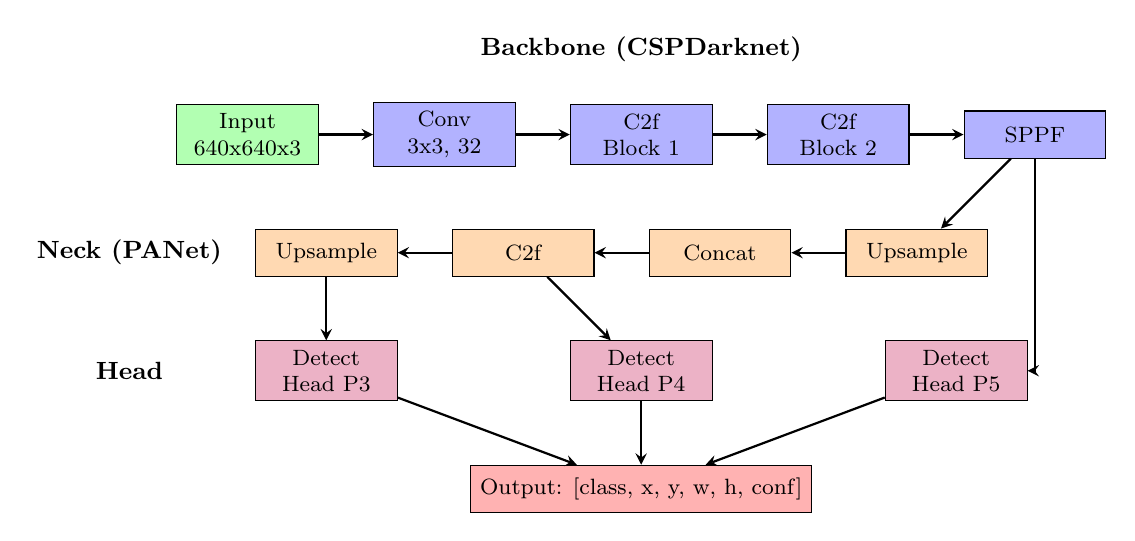
\begin{tikzpicture}[
    node distance=0.8cm,
    box/.style={rectangle, draw, fill=blue!20, minimum width=1.8cm, minimum height=0.6cm, align=center, font=\footnotesize},
    arrow/.style={->, thick, >=stealth}
]

% Input
\node[box, fill=green!30] (input) at (0, 0) {Input\\640x640x3};

% Backbone
\node[box, fill=blue!30] (conv1) at (2.5, 0) {Conv\\3x3, 32};
\node[box, fill=blue!30] (c2f1) at (5, 0) {C2f\\Block 1};
\node[box, fill=blue!30] (c2f2) at (7.5, 0) {C2f\\Block 2};
\node[box, fill=blue!30] (sppf) at (10, 0) {SPPF};

% Neck
\node[box, fill=orange!30] (upsample1) at (8.5, -1.5) {Upsample};
\node[box, fill=orange!30] (concat1) at (6, -1.5) {Concat};
\node[box, fill=orange!30] (c2f4) at (3.5, -1.5) {C2f};
\node[box, fill=orange!30] (upsample2) at (1, -1.5) {Upsample};

% Head
\node[box, fill=purple!30] (head1) at (1, -3) {Detect\\Head P3};
\node[box, fill=purple!30] (head2) at (5, -3) {Detect\\Head P4};
\node[box, fill=purple!30] (head3) at (9, -3) {Detect\\Head P5};

% Output
\node[box, fill=red!30] (output) at (5, -4.5) {Output: [class, x, y, w, h, conf]};

% Arrows - Backbone
\draw[arrow] (input) -- (conv1);
\draw[arrow] (conv1) -- (c2f1);
\draw[arrow] (c2f1) -- (c2f2);
\draw[arrow] (c2f2) -- (sppf);

% Arrows - Neck
\draw[arrow] (sppf) -- (upsample1);
\draw[arrow] (upsample1) -- (concat1);
\draw[arrow] (concat1) -- (c2f4);
\draw[arrow] (c2f4) -- (upsample2);

% Arrows - to heads
\draw[arrow] (upsample2) -- (head1);
\draw[arrow] (c2f4) -- (head2);
\draw[arrow] (sppf) |- (head3);

% Arrows - to output
\draw[arrow] (head1) -- (output);
\draw[arrow] (head2) -- (output);
\draw[arrow] (head3) -- (output);

% Labels
\node[font=\small\bfseries, above] at (5, 0.8) {Backbone (CSPDarknet)};
\node[font=\small\bfseries] at (-1.5, -1.5) {Neck (PANet)};
\node[font=\small\bfseries] at (-1.5, -3) {Head};

\end{tikzpicture}
\caption{YOLOv8 архитектурын бүтэц}
\label{fig:yolov8_architecture}
\end{figure}

YOLOv8 загварын дотоод бүтцийг авч үзвэл үндсэндээ гурван хэсгээс бүрдэнэ:

\subsection{Backbone (Сээр нуруу)}
CSPDarknet53 архитектурын сайжруулсан хувилбарыг ашигладаг. Оролтын зургаас үндсэн онцлог шинж чанаруудыг (өнгө, хэлбэр, зураас) татаад авдаг хэсэг. Шинэ загварт C3 модулийг C2f модулиар сольсноор:
\begin{itemize}
    \item Параметрийн тоо багассан
    \item Градиентийн урсгал сайжирсан
    \item Тооцооллын хурд нэмэгдсэн
\end{itemize}

\subsection{Neck (Хүзүү)}
PANet (Path Aggregation Network) маягийн бүтцийг ашиглан Backbone-оос ирсэн өөр өөр нягтаршлын түвшний онцлогуудтай давхаргуудыг хооронд нь холбож нэгтгэдэг. Ингэснээр:
\begin{itemize}
    \item Жижиг объектуудыг (жишээ нь зай) илрүүлэх чадвар дээшилдэг
    \item Том объектуудыг нэгэн зэрэг алдаагүй таних
    \item Multi-scale feature fusion хийгддэг
\end{itemize}

\subsection{Head (Толгой)}
YOLOv8 нь Anchor-Free (зангуугүй) толгойтой болсон. Хуучин шиг урьдчилаад зохиомол anchor box-уудын хэмжээг тооцдоггүйгээр зургийн аль хэсэгт объектын төв байна, түүний хил хязгаар нь хаана хүртэл байна гэдгийг Decoupled Head ашиглан байршил болон ангиллыг тус тусад нь тооцож гаргадаг. Энэхүү хандлага нь Vaswani нарын Attention механизмын санаанаас үндэслэлтэй \cite{attention_mechanism}.

%==============================================================================
% 2.8 АЛДААНЫ ФУНКЦ
%==============================================================================
\section{Алдааны функц (Loss Function)}

Уг загвар нь сургалтын үеийн алдааг тооцоолохдоо хэд хэдэн алдааны функцийн нийлбэрийг ашигладаг:

\begin{equation}
    \mathcal{L}_{total} = \lambda_{box} \cdot \mathcal{L}_{box} + \lambda_{cls} \cdot \mathcal{L}_{cls} + \lambda_{dfl} \cdot \mathcal{L}_{dfl}
\end{equation}

Энд:
\begin{itemize}
    \item $\mathcal{L}_{box}$ --- CIoU (Complete Intersection over Union) loss: Bounding box-ийн нарийвчлалыг хэмждэг
    \item $\mathcal{L}_{cls}$ --- Binary Cross Entropy loss: Ангиллыг зөв таамагласан эсэхийг хэмждэг
    \item $\mathcal{L}_{dfl}$ --- Distribution Focal Loss: Объектын ирмэг хаагуур өнгөрч байгааг нарийвчлан тооцоолдог
    \item $\lambda_{box}, \lambda_{cls}, \lambda_{dfl}$ --- Жингийн коэффициентүүд
\end{itemize}

\textbf{CIoU Loss:}
\begin{equation}
    \mathcal{L}_{CIoU} = 1 - IoU + \frac{\rho^2(b, b^{gt})}{c^2} + \alpha v
\end{equation}
Энд $\rho$ нь төвүүдийн Евклидийн зай, $c$ нь хоёр хайрцгийг бүрхсэн хамгийн жижиг тэгш өнцөгтийн диагональ, $\alpha$ ба $v$ нь харьцааны тэнцвэржүүлэгч параметрүүд юм.

%==============================================================================
% 2.9 АУДИТ АЛГОРИТМ
%==============================================================================
\section{Аудит хийх алгоритм ба математик загварчлал}

Илрүүлэлт (Detection) амжилттай хийгдэж, зураг дээрээс бараануудыг олсны дараа аудитын хөдөлгүүр (Audit Engine) ажиллаж эхэлнэ. Энэхүү модулийн гол зорилго нь ``Олдсон'' барааг ``Байх ёстой'' мэдээлэлтэй автоматаар тулгаж, логик дүгнэлт гаргах явдал юм.

\subsection{Математик тодорхойлолт}

Тухайн лангуунд бүртгэгдсэн, хүлээгдэж буй (Expected) бараануудын багцыг $E$, зургаас танигдсан (Detected) бараануудын багцыг $D$ гэж үзье.

\textbf{Хүлээгдэж буй нийт тоо:}
\begin{equation}
    E_{total} = \sum_{i \in Items} E_i
\end{equation}
Энд $E_i$ нь $i$-р барааны хүлээгдэж буй тоо хэмжээ.

\textbf{Нийт таарсан зөв тоо:}
\begin{equation}
    M_{total} = \sum_{i \in Items} \min(D_i, E_i)
\end{equation}
Энд $D_i$ нь зургаас илрүүлж тоолсон тухайн барааны илэрцийн тоо.

\textbf{Тохирлын хувь (Match Rate):}
\begin{equation}
    R_{match} = \frac{M_{total}}{E_{total}} \times 100\%
\end{equation}

\textbf{Зөрүү (Discrepancy):}
\begin{equation}
    \Delta_i = D_i - E_i
\end{equation}

\subsection{Аудитын статусын тодорхойлолт}

\begin{figure}[H]
\centering
\begin{tikzpicture}[
    node distance=2cm,
    decision/.style={diamond, draw, fill=yellow!30, minimum width=2cm, minimum height=1cm, align=center, inner sep=0pt, font=\footnotesize},
    process/.style={rectangle, draw, fill=blue!20, minimum width=2cm, minimum height=0.8cm, align=center, rounded corners, font=\footnotesize},
    result/.style={rectangle, draw, minimum width=2cm, minimum height=0.8cm, align=center, rounded corners, font=\footnotesize},
    arrow/.style={->, thick, >=stealth}
]

% Start
\node[process] (start) at (0, 0) {Илрүүлэлт\\хийх};

% Calculate
\node[process] (calc) at (0, -1.5) {$R_{match}$\\тооцоолох};

% Decision 1
\node[decision] (d1) at (0, -3.5) {$R_{match}$\\$= 100\%$?};

% Decision 2
\node[decision] (d2) at (3.5, -3.5) {$R_{match}$\\$\geq 80\%$?};

% Results
\node[result, fill=green!40] (pass) at (-3, -5.5) {\textbf{PASS}\\Амжилттай};
\node[result, fill=yellow!40] (warn) at (1, -5.5) {\textbf{WARNING}\\Анхааруулга};
\node[result, fill=red!40] (fail) at (5, -5.5) {\textbf{FAIL}\\Бүтэлгүйтсэн};

% Arrows
\draw[arrow] (start) -- (calc);
\draw[arrow] (calc) -- (d1);
\draw[arrow] (d1) -- node[left, font=\scriptsize] {Тийм} (pass);
\draw[arrow] (d1) -- node[above, font=\scriptsize] {Үгүй} (d2);
\draw[arrow] (d2) -- node[left, font=\scriptsize] {Тийм} (warn);
\draw[arrow] (d2) -- node[right, font=\scriptsize] {Үгүй} (fail);

\end{tikzpicture}
\caption{Аудитын шийдвэр гаргах алгоритмын урсгал}
\label{fig:audit_flowchart}
\end{figure}

Аудитын эцсийн статусыг дараах байдлаар тодорхойлов:

\begin{description}
    \item[\textbf{PASS (Амжилттай):}] $R_{match} = 100\%$ --- Бүх хүлээгдэж байсан бараанууд яг бодит байдал дээрхтэйгээ таарсан. Ногоон төлөв.
    
    \item[\textbf{WARNING (Анхааруулга):}] $80\% \leq R_{match} < 100\%$ --- Цөөн хэдэн бараа дутсан. Шар төлөв. Лангууны хойд талд бараа нуугдсан эсвэл түр зуур зарагдаад цөөрсөн үед ийм дохио ирнэ.
    
    \item[\textbf{FAIL (Бүтэлгүйтсэн):}] $R_{match} < 80\%$ --- Өрөгдвөл зохих бараанууд огт тавигдаагүй, эсвэл өөр төрлийн бараанууд олноор орж ирсэн. Улаан төлөв.
\end{description}

\subsection{Нэмэлт зөрүүний илрүүлэлт}

\textbf{Дутуу бараанууд (Missing products):}
\begin{equation}
    Missing = \{i \in E : D_i = 0\}
\end{equation}

\textbf{Илүү бараанууд (Extra products):}
\begin{equation}
    Extra = \{i \in D : i \notin E\}
\end{equation}

%==============================================================================
% 2.10 API ENDPOINTS
%==============================================================================
\section{Сервер болон хэрэглэгчийн талын архитектурын онцлогууд}

\subsection{FastAPI Backend}
FastAPI нь Python хэлний төрлийн заагч (type hints) дээр тулгуурлаж ажилладаг бөгөөд:
\begin{itemize}
    \item Кодчиллын үед гарах алдааг бууруулдаг
    \item \texttt{asyncio} технологийг ашиглаж I/O үйлдлүүдийн үед серверийн ачааллыг түгжихгүй
    \item Бусад хэрэглэгчдийн хүсэлтийг давхар шийдвэрлэх (Concurrency) боломжтой
\end{itemize}

\begin{table}[H]
\centering
\caption{API Endpoint-уудын жагсаалт}
\label{tab:api_endpoints}
\begin{tabular}{|l|l|p{6cm}|}
\hline
\textbf{Арга} & \textbf{Endpoint} & \textbf{Тайлбар} \\
\hline
POST & /api/detection/detect & Зураг хүлээн авч илрүүлэлт хийх \\
\hline
GET & /api/detection/history & Илрүүлэлтийн түүх харах \\
\hline
POST & /api/audit/run & Аудит хийх \\
\hline
GET & /api/audit/history & Аудитын түүх харах \\
\hline
GET & /api/audit/stats & Статистик мэдээлэл \\
\hline
GET & /api/products/ & Бүртгэлтэй бараанууд \\
\hline
POST & /api/products/ & Шинэ бараа бүртгэх \\
\hline
PUT & /api/products/\{name\} & Бараа засварлах \\
\hline
DELETE & /api/products/\{name\} & Бараа устгах \\
\hline
\end{tabular}
\end{table}

\subsection{Flutter Frontend}
Flutter нь бүх элементүүдийг Widget гэж үздэг. Аппликейшний интерфейсийн хөгжүүлэлтэд:
\begin{itemize}
    \item UI ба Бизнес Логикийг хооронд нь тусгаарлах (MVVM архитектур)
    \item Provider State Management ашиглан төлөв удирдах
    \item Сүлжээний алдаа, өгөгдөл шинэчлэгдэх явцуудыг нэг доороос удирдах
\end{itemize}

\begin{figure}[H]
\centering
\begin{tikzpicture}[
    node distance=1cm,
    box/.style={rectangle, draw, fill=blue!20, minimum width=3cm, minimum height=0.8cm, align=center, rounded corners},
    arrow/.style={<->, thick, >=stealth}
]

% Layers
\node[box, fill=cyan!30] (ui) at (0, 2) {UI Layer\\(Widgets)};
\node[box, fill=green!30] (state) at (0, 0.5) {State Management\\(Provider)};
\node[box, fill=orange!30] (service) at (0, -1) {Service Layer\\(API calls)};
\node[box, fill=purple!30] (api) at (0, -2.5) {REST API\\(HTTP)};

% Arrows
\draw[arrow] (ui) -- (state);
\draw[arrow] (state) -- (service);
\draw[arrow] (service) -- (api);

% Labels
\node[font=\footnotesize, right] at (2, 2) {Дэлгэцийн харагдах байдал};
\node[font=\footnotesize, right] at (2, 0.5) {Төлөв удирдлага};
\node[font=\footnotesize, right] at (2, -1) {Сүлжээний хүсэлт};
\node[font=\footnotesize, right] at (2, -2.5) {Сервертэй холбогдох};

\end{tikzpicture}
\caption{Flutter аппликейшний давхаргат архитектур}
\label{fig:flutter_architecture}
\end{figure}

%==============================================================================
% 2.11 ӨГӨГДЛИЙН УРСГАЛ
%==============================================================================
\section{Өгөгдлийн урсгал (Data Flow)}

Системийн бүрэн өгөгдлийн урсгалыг дараах диаграммаар харуулав:

\begin{figure}[H]
\centering
\begin{tikzpicture}[
    node distance=0.8cm,
    step/.style={rectangle, draw, fill=blue!20, minimum width=2.5cm, minimum height=0.6cm, align=center, rounded corners, font=\footnotesize},
    arrow/.style={->, thick, >=stealth}
]

% Steps
\node[step, fill=cyan!30] (s1) at (0, 0) {1. Зураг авах};
\node[step, fill=cyan!30] (s2) at (3.5, 0) {2. Сервер рүү\\илгээх};
\node[step, fill=green!30] (s3) at (7, 0) {3. Зураг\\хадгалах};
\node[step, fill=purple!30] (s4) at (10.5, 0) {4. YOLOv8\\илрүүлэлт};

\node[step, fill=orange!30] (s5) at (10.5, -1.5) {5. MongoDB\\хадгалах};
\node[step, fill=yellow!30] (s6) at (7, -1.5) {6. Аудит\\хийх};
\node[step, fill=red!30] (s7) at (3.5, -1.5) {7. Статус\\тодорхойлох};
\node[step, fill=cyan!30] (s8) at (0, -1.5) {8. Үр дүн\\харуулах};

% Arrows
\draw[arrow] (s1) -- (s2);
\draw[arrow] (s2) -- (s3);
\draw[arrow] (s3) -- (s4);
\draw[arrow] (s4) -- (s5);
\draw[arrow] (s5) -- (s6);
\draw[arrow] (s6) -- (s7);
\draw[arrow] (s7) -- (s8);

\end{tikzpicture}
\caption{Системийн өгөгдлийн урсгал}
\label{fig:data_flow}
\end{figure}

\end{document}
